\documentclass[12pt]{article}
\usepackage[utf8]{inputenc}
\usepackage{hyperref}
\usepackage{listings}
\usepackage{xcolor}
\usepackage{geometry}
\usepackage{graphicx} % For including graphics
\usepackage{minted} % For advanced code listings
\usepackage{listings-solidity}  % Include Solidity highlighting
\usepackage{amsmath, amssymb, amsfonts} % For mathematical equations


% Define a custom minted style (optional)
\usemintedstyle{colorful} % You can choose from various styles like 'monokai', 'tango', 'colorful', etc.

% Custom color setup
\definecolor{bashtextcolor}{RGB}{0, 0, 0} % Define black color

% Define a new command for inline code using minted
\newcommand{\codeinline}[1]{\mintinline{text}{#1}}

\geometry{a4paper, margin=1in}

\title{Smart Contracts Exercise 08: \\ Maximal Extractable Value}
\author{}
\date{}

% Define a new command for inline code with a dark background
\newcommand{\codeblack}[1]{%
  \texttt{\colorbox{black!7}{\textcolor{black}{#1}}}%
}

% Define a new command for inline code with a dark background
\newcommand{\codegrey}[1]{%
  \texttt{\colorbox{black!4}{\textcolor{black}{#1}}}%
}

% Define custom colors (optional)
\definecolor{myURLColor}{RGB}{0, 102, 204} % Example: A shade of blue

\hypersetup{
    colorlinks=true,        % Enable colored links
    linkcolor=blue,         % Color for internal links (e.g., \ref, \cite)
    citecolor=blue,         % Color for citations
    filecolor=magenta,      % Color for file links
    urlcolor=myURLColor     % Color for external URLs
}

% Define a style for code listings
\lstdefinestyle{mystyle}{
    backgroundcolor=\color{lightgray!20},   
    commentstyle=\color{green!50!black},
    keywordstyle=\color{blue},
    numberstyle=\tiny\color{gray},
    stringstyle=\color{red},
    basicstyle=\ttfamily\footnotesize,
    breakatwhitespace=false,         
    breaklines=true,                 
    captionpos=b,                    
    keepspaces=true,                 
    numbers=left,                    
    numbersep=5pt,                  
    showspaces=false,                
    showstringspaces=false,
    showtabs=false,                  
    tabsize=2
}

\lstset{style=mystyle}
% Adding package for header and footer
\usepackage{fancyhdr}
\pagestyle{fancy}

% Define header and footer
\fancyhf{} % Clear current settings
\fancyhead[L]{Smart Contracts Exercise 08} % Left header
\fancyhead[R]{\thepage} % Right header with page number

\renewcommand{\headrulewidth}{0.4pt} % Line below header
% \renewcommand{\footrulewidth}{0.4pt} % Line above footer

\begin{document}

\maketitle
\section{Introduction}

We first encountered frontrunning in Exercise 3: ERC20 - CTUToken. Frontrunning falls under the more general term known as MEV - Maximal Extractable Value. MEV has become a very important topic for Ethereum that needs to be addressed. In this exercise, we will examine this phenomenon in more detail. We'll explore additional MEV techniques and examples, such as DEX arbitrage, liquidations, sandwich trading, and more. An important topic of the exercise will also be calculating transaction fees, gas, and EIP-1559. In the practical exercises, you will try frontrunning an NFT auction and executing a sandwich attack on a DEX yourself. Finally, we'll look at how MEV is being solved today and introduce terms such as Proposer-Builder Separation and Builder APIs.

\subsection*{Project Setup}

You have two options for working with this exercise. Using docker container or local installation. Choose the one that best fits your preferences.

\subsection{Using Docker with VS Code}

This option uses Docker to create a development environment with all the necessary tools and dependencies pre-installed.

\subsubsection*{Prerequisites:}

\begin{itemize}
    \item \textbf{\href{https://www.docker.com/products/docker-desktop}{Docker}} - A platform for developing, shipping, and running applications in containers.
    \item \textbf{\href{https://code.visualstudio.com/}{Visual Studio Code}} - A lightweight but powerful source code editor.
    \item \textbf{\href{https://marketplace.visualstudio.com/items?itemName=ms-vscode-remote.remote-containers}{Dev Containers}} - An extension to VS Code that lets you use a Docker container as a full-featured development environment.
\end{itemize}

\subsubsection*{Setting Up the Project:}

\begin{enumerate}
  \item Visit the following \href{https://gitlab.fel.cvut.cz/radovluk/smart-contracts-exercises/-/tree/main/08-Maximal-Extractable-Value/task/task-code}{GitLab repository} and clone it to your local machine.
  \item Open the repository folder in VS Code.
  \item When prompted, click "Reopen in Container" or use the command palette (F1) and run \codegrey{Dev Containers: Reopen in Container}.
\end{enumerate}

\subsection{Local Setup}

If you prefer working directly on your machine without Docker, you can set up the development environment locally.

\subsubsection*{Prerequisites}
\begin{itemize}
    \item \textbf{Node.js} - \url{https://nodejs.org/en/} - An open-source, cross-platform, back-end JavaScript runtime environment that runs on the V8 engine and executes JavaScript code outside a web browser.
    \item \textbf{NPM}: Node Package Manager, which comes with Node.js.
\end{itemize}

\noindent
Open your terminal and run the following commands to verify the installations:

\begin{minted}[bgcolor=gray!5, fontsize=\footnotesize]{bash}
$ node -v
$ npm -v
\end{minted}

Both commands should return the installed version numbers of Node.js and NPM respectively. Node.js provides the runtime environment required to execute JavaScript-based tools like Hardhat, while NPM is used to manage the packages and dependencies needed for development.

\subsubsection*{Setting Up the Project}

\begin{enumerate}
    \item Visit the following \href{https://gitlab.fel.cvut.cz/radovluk/smart-contracts-exercises/-/tree/main/08-Maximal-Extractable-Value/task/task-code}{GitLab repository} and clone it to your local machine.
    \item Open a terminal and navigate to the project directory.
    \item Install the project dependencies by running \codegrey{npm install}.
\end{enumerate}

\section{Maximal Extractable Value (MEV)}

MEV stands for Maximal Extractable Value, which refers to the maximum value that can be extracted during block production in addition to the standard block rewards and gas fees. This value can be extracted by adding transactions to a block, removing transactions from it, or changing the order of transactions within the block. Originally, the acronym stood for "Miner Extractable Value," but since \href{https://ethereum.org/en/roadmap/merge/}{the Merge} replaced miners with validators, it's now known as "Maximal Extractable Value."

\subsection*{Types of MEV}

Several types of MEV extraction can be identified:

\begin{enumerate}
  \item \textbf{Frontrunning}: An attacker observes a pending transaction in the mempool and submits their own transaction to be included in the block before the original transaction.
  \item \textbf{Backrunning}: An attacker observes a pending transaction in the mempool and submits their own transaction to be included in the block immediately after the original transaction.
  \item \textbf{Sandwich Attack}: An attacker places two transactions around the victim's transaction - one before and one after.
  \item \textbf{Transaction Censorship}: An attacker omits a transaction from the block to prevent it from being executed.
\end{enumerate}

\begin{figure}[H]
  \centering
  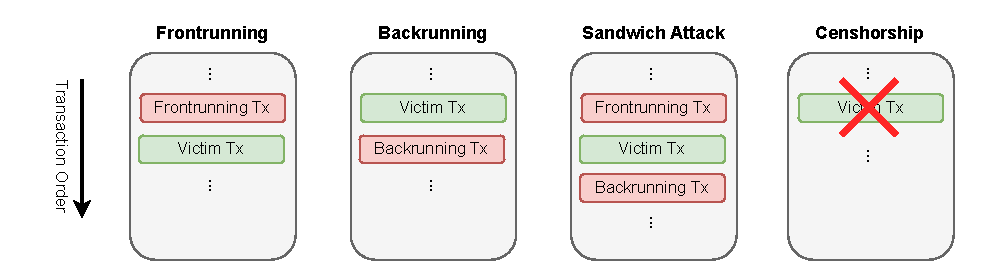
\includegraphics[width=1\textwidth]{MEV.pdf}
  % \caption{Frontrunning Attack}
  \label{fig:sandwich}
\end{figure}

\noindent
To better understand why these techniques are profitable for attackers, let's examine some specific examples:

\subsubsection*{DEX Arbitrage} If two DEXes offer tokens at different prices, someone can include a transaction in a block that buys tokens on one DEX and sells them at a higher price on another DEX. In this situation, the block creator can exploit this opportunity to profit from the arbitrage. Here's an \href{https://etherscan.io/tx/0x5e1657ef0e9be9bc72efefe59a2528d0d730d478cfc9e6cdd09af9f997bb3ef4}{example of such transaction}.

\subsubsection*{Sandwich Attack}
If someone wants to exchange a large amount of a specific token on a DEX, an attacker can add transactions that buy tokens before the large transaction and sell them afterward. Thanks to how DEXes set prices using the constant product formula ($x \cdot y = k$), this approach can be profitable. The process is detailed in Table~\ref{tab:sandwich-attack} and illustrated in Figure~\ref{fig:sandwich}.

\begin{table}[h]
  \centering
  \footnotesize
  \begin{tabular}{|p{0.05\textwidth}|p{0.2\textwidth}|p{0.6\textwidth}|}
  \hline
  \textbf{Step} & \textbf{Action} & \textbf{Description} \\
  \hline
  1 & Alice creates transaction & Alice submits transaction Tx1 (\$\$) to the mempool to swap a large amount of tokens on a DEX. \\
  \hline
  2 & Bob monitors mempool & Bob identifies Alice's pending transaction as an opportunity for a sandwich attack. \\
  \hline
  3 & Bob creates frontrun & Bob submits transaction Tx2 (\$\$\$) with higher gas fees to buy the same tokens before Alice's swap executes. \\
  \hline
  4 & Token price increases & After Bob's purchase, token price increases according to $P_{\text{new}} = \frac{y - \Delta y}{x + \Delta x}$ where $\Delta x$ is Bob's input and $\Delta y$ is tokens received. \\
  \hline
  5 & Alice's transaction executes & Alice's swap executes at worse price conditions due to Bob's prior purchase, receiving fewer tokens than expected. \\
  \hline
  6 & Token price increases further & Alice's large swap further increases the token price due to the constant product formula, making Bob's tokens worth more. \\
  \hline
  7 & Bob executes backrun & Bob's transaction Tx3 (\$) sells the tokens at the higher price caused by Alice's large swap. \\
  \hline
  8 & Bob profits & Bob profits from the price difference: $\text{Profit} = \text{Sell proceeds} - \text{Purchase cost} - \text{Gas fees}$. \\
  \hline
  9 & Price impact on Alice & Alice experiences negative price impact, receiving fewer tokens than expected in a fair market. \\
  \hline
  \end{tabular}
  \caption{Sandwich Attack Mechanism on a Decentralized Exchange (DEX). The attack exploits the AMM pricing formula and transaction ordering. For visual representation, see Figure~\ref{fig:sandwich}.}
  \label{tab:sandwich-attack}
\end{table}

\begin{figure}[H]
  \centering
  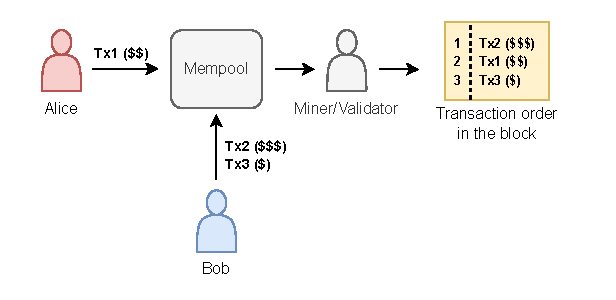
\includegraphics[width=0.75\textwidth]{sandwich.pdf}
  \caption{Sandwich Attack visualization showing how transactions are ordered in the mempool and block. The price changes follow the AMM constant product formula ($x \cdot y = k$) where $x$ and $y$ are token reserves.}
  \label{fig:sandwich}
\end{figure}

\subsubsection*{Liquiditations} When borrowers in lending protocols fall below required collateralization ratios, their positions become eligible for liquidation. Block producers can prioritize their own liquidation transactions, allowing them to claim the liquidation rewards and discounted collateral before other participants. This gives them an advantage in capturing value from distressed positions.

\subsubsection*{Other MEVs}
MEV opportunities are derived from smart contracts and their functionalities. Consider, for example, the auction from the previous exercise. If the block creator is interested in the auctioned item, they can simply add their transaction at the end of the auction, placing it before the transaction that ends the auction.

Consider this example where a MEV searcher purchased every single Cryptopunk at the floor price for \$7 million: \href{https://etherscan.io/address/0x650dCdEB6ecF05aE3CAF30A70966E2F395d5E9E5}{Searcher's address}.

\medskip
\noindent
More about MEV:
\begin{itemize}
  \item \textbf{Read:} \href{https://ethereum.org/en/developers/docs/mev/}{Maximal extractable value (MEV)}
  \item \textbf{Animated Video:} \href{https://www.youtube.com/watch?v=F9IuBZGseFQ}{Decoding MEV: Past, Present, Future}
  \item \textbf{MEV Real Time Detection:} \href{https://eigenphi.io/}{https://eigenphi.io/}
\end{itemize}

% \section{EIP-1559: Transaction Pricing Mechanism}

% Ethereum Improvement Proposal 1559 (EIP-1559) introduced a new transaction pricing mechanism designed to make fee estimation more predictable and improve user experience.

% \subsection{How Gas Pricing Works}

% Before EIP-1559, users would specify a \codegrey{gasPrice} which was a simple auction system - higher gas price meant higher priority. With EIP-1559, this changed to a more complex but predictable system.

% \subsubsection*{EIP-1559 Transaction Structure}

% Under EIP-1559, transactions include:

% \begin{itemize}
%     \item \codegrey{maxFeePerGas}: The maximum total fee the user is willing to pay per unit of gas
%     \item \codegrey{maxPriorityFeePerGas}: The maximum tip the user is willing to pay to validators
%     \item \codegrey{gasLimit}: The maximum amount of gas the transaction can consume
% \end{itemize}

% \subsubsection*{Base Fee}

% Every block has a \codegrey{baseFee} which is burned (removed from circulation). The base fee adjusts automatically based on network demand:

% \begin{itemize}
%     \item If blocks are more than 50\% full, the base fee increases by up to 12.5\% per block
%     \item If blocks are less than 50\% full, the base fee decreases by up to 12.5\% per block
% \end{itemize}

% This mechanism helps maintain block space demand around the target gas limit.

% \subsubsection*{Total Fee Calculation}

% The actual fee per gas paid by a transaction is calculated as:
% \begin{equation}
% \text{Fee per gas} = \text{baseFee} + \min(\text{maxPriorityFeePerGas}, \text{maxFeePerGas} - \text{baseFee})
% \end{equation}

% Where:
% \begin{itemize}
%     \item \codegrey{baseFee} is burned (removed from circulation)
%     \item The priority fee (or tip) goes to the validator as an incentive
% \end{itemize}

% \subsubsection*{When Transactions Fail}

% \begin{itemize}
%     \item If \codegrey{maxFeePerGas < baseFee}: Transaction becomes invalid and will be rejected
%     \item If \codegrey{baseFee + maxPriorityFeePerGas > maxFeePerGas}: Priority fee is reduced to \codegrey{maxFeePerGas - baseFee}
% \end{itemize}

% \subsubsection*{Total Transaction Fee}

% The total fee paid for a transaction is:
% \begin{equation}
% \text{Total Fee} = \text{Gas Used} \times (\text{Base Fee} + \text{Priority Fee})
% \end{equation}

\pagebreak
\section{Task}

\subsection*{Task 1: NFT Auction Frontrunning}
Another rare NFT from the FEL Student Collection is up for auction - specifically, a student from the OES program caught sleepwalking with a laptop (apparently a common occurrence during exam season). This time the auction is well-protected against DoS attacks and fully implements the push-over-pull pattern from the previous exercise. The bidding has already reached 1.5 ETH. You don't want to place bids until the last possible moment to avoid being outbid. You've been monitoring the public mempool, waiting for the event organizer to call the \codegrey{endAuction()} function so you can be the final bidder. 

With 1.51 ETH in your wallet and a strong desire for this NFT, you're watching closely for your chance to place a bid just before the auction officially ends...

\begin{figure}[H]
  \centering
  \begin{minipage}{0.3\textwidth}
    
\includegraphics[width=\textwidth]{NFTs/oes-student-nft.pdf}
  \end{minipage}
\end{figure}

\medskip
\noindent
\textbf{Your Mission:}
\begin{itemize}
    \item Monitor the mempool for the \codegrey{endAuction()} transaction
    \item Gain the OES student NFT
\end{itemize}

\noindent
Code your solution in the \texttt{test/NFTAuction.js} file. Use the player account only. Verify your solution by running:

\begin{minted}[bgcolor=gray!5, fontsize=\footnotesize]{bash}
$ npm run auction
\end{minted}

\noindent
Files that are relevant for this challenge:
\begin{itemize}
\item test/\textbf{NFTAuction.js}: The test file where you should code your solution.
\item contracts/\textbf{NFTAuction.sol}: The improved auction contract.
\item contracts/\textbf{FELStudentNFT.sol}: The NFT collection contract.
\end{itemize}

\subsection*{Task 2: Sandwich Attack on a DEX}

You've been monitoring the mempool and spot a juicy opportunity: someone (let's call them "Innocent Victim") is about to swap a massive 20 ETH for USDC tokens on SimpleDEX. With your knowledge of DeFi and MEV, you realize this is a perfect opportunity for a sandwich attack.

You have 15 ETH at your disposal, and your blockchain professor would be so proud to see you apply your learnings in real life (or maybe not...).

\medskip
\noindent
\textbf{Your Mission:}
\begin{itemize}
  \item Execute a sandwich attack on the victim's transaction
  \item Make a profit of at least 1 ETH from this MEV extraction
\end{itemize}

\noindent
Code your solution in the \texttt{test/SandwichAttack.js} file. Use the player account for your transactions. Verify your solution by running:

\begin{minted}[bgcolor=gray!5, fontsize=\footnotesize]{bash}
$ npm run sandwich
\end{minted}

\noindent
Files that are relevant for this challenge:
\begin{itemize}
\item test/\textbf{SandwichAttack.js}: The test file where you should code your solution.
\item contracts/\textbf{SimpleDEX.sol}: A decentralized exchange with a one liquidity pool containing 500 ETH and 1000000 USDC.
\item contracts/\textbf{USDCToken.sol}: An ERC20 token representing simplified version of USDC.
\end{itemize}

\end{document}